% !TEX encoding = UTF-8 Unicode
%!TEX root = thesis.tex
% !TEX spellcheck = en-US
%%=========================================
\section{Experiment 3}
When using an evolved cross-adaptive audio effect in a live performance, a performer may want to use it in an expressive way. For example, if the performer is a drummer, he can vary the intensity of the drum hits. For the cross-adaptive audio effect to handle this, it needs to be trained on all the different intensities of the drum hits. If an extensive recording is available, that is fine. However, if the available target sound is short or lacks sufficient variation, one can harness the concept of data augmentation to create artificial variations of that sound. If one uses that sound instead, the evolved effect will typically be more capable of dealing with the generated variations. This experiment is about testing the author's implementation of data augmentation and the ability to apply evolved cross-adaptive audio effects to unseen sounds.

\subsection{Configuration}

\begin{center}
\begin{longtable}{p{5cm} p{7cm}}
\caption[Experiment configuration]{Experiment configuration} \label{tab:exp3_configuration} \\

\hline \multicolumn{1}{l}{\textbf{Parameter}} & \multicolumn{1}{l}{\textbf{Value}} \\ \hline 
\endfirsthead

\multicolumn{2}{c}%
{{\bfseries \tablename\ \thetable{} -- continued from previous page}} \\
\hline \multicolumn{1}{l}{\textbf{Parameter}} & \multicolumn{1}{l}{\textbf{Value}} \\ \hline 
\endhead

\hline \multicolumn{2}{r}{{Continued on next page}} \\ \hline
\endfoot

\hline \hline
\endlastfoot

Number of generations & 20 \\
\midrule
Target sound (training) & Drum loop with bass drum, snare drum, clap and hihat (figure \ref{fig:exp3_waveforms}) \\
\midrule
Target sound (validation) & Snare roll (rapid snare drum hits) with ascending pitch and amplitude (figure \ref{fig:exp3_waveforms}) \\
\midrule
Input sound & White noise \\
\midrule
Effect & Distortion and resonant low-pass filter \\
\midrule
Audio features & Root Mean Square (RMS) and spectral centroid \\
\midrule
Number of runs & 40 per configuration \\
\end{longtable}
\end{center}

\begin{figure}[H]
    \centering
    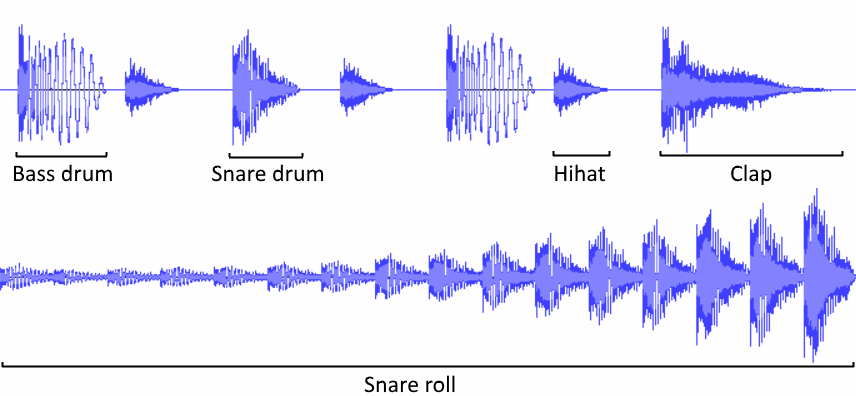
\includegraphics[width=1.0\textwidth]{exp3_waveforms}
    \caption{Waveform of training sound (top) and validation sound (bottom)}
    \label{fig:exp3_waveforms}
\end{figure}

The augmented variant of the training sound was created by repeating the sound 8 times, with variations in playback speed and gain for each repetition. The playback speed and gain are obtained by sampling from a gaussian distribution with standard deviations of $0.3$ and $0.5$, respectively.

Runs with three different target sounds (training sound, augmented training sound and validation sound) will be compared. The resulting effects are applied to the validation sound, and fitness values are measured. The neural networks trained on the validation sound are of course expected to be yield the highest fitness scores when tested on the validation sound. That configuration is included for comparison, as an upper bound estimate.

\subsection{Results and Evaluation}
Figure \ref{fig:exp3_fitness_box} shows that neural networks trained on an augmented variant of the training sound generalize better than neural networks trained on the nonaugmented training sound. In other words, the resulting audio effects becomes better at dealing with nuances of the situations in the training sound. There's a trade-off, however: Training on an augmented sound requires more computational time because there's more data to process. This may not be a problem, because training can be done before live performance starts.

\begin{figure}[H]
    \centering
    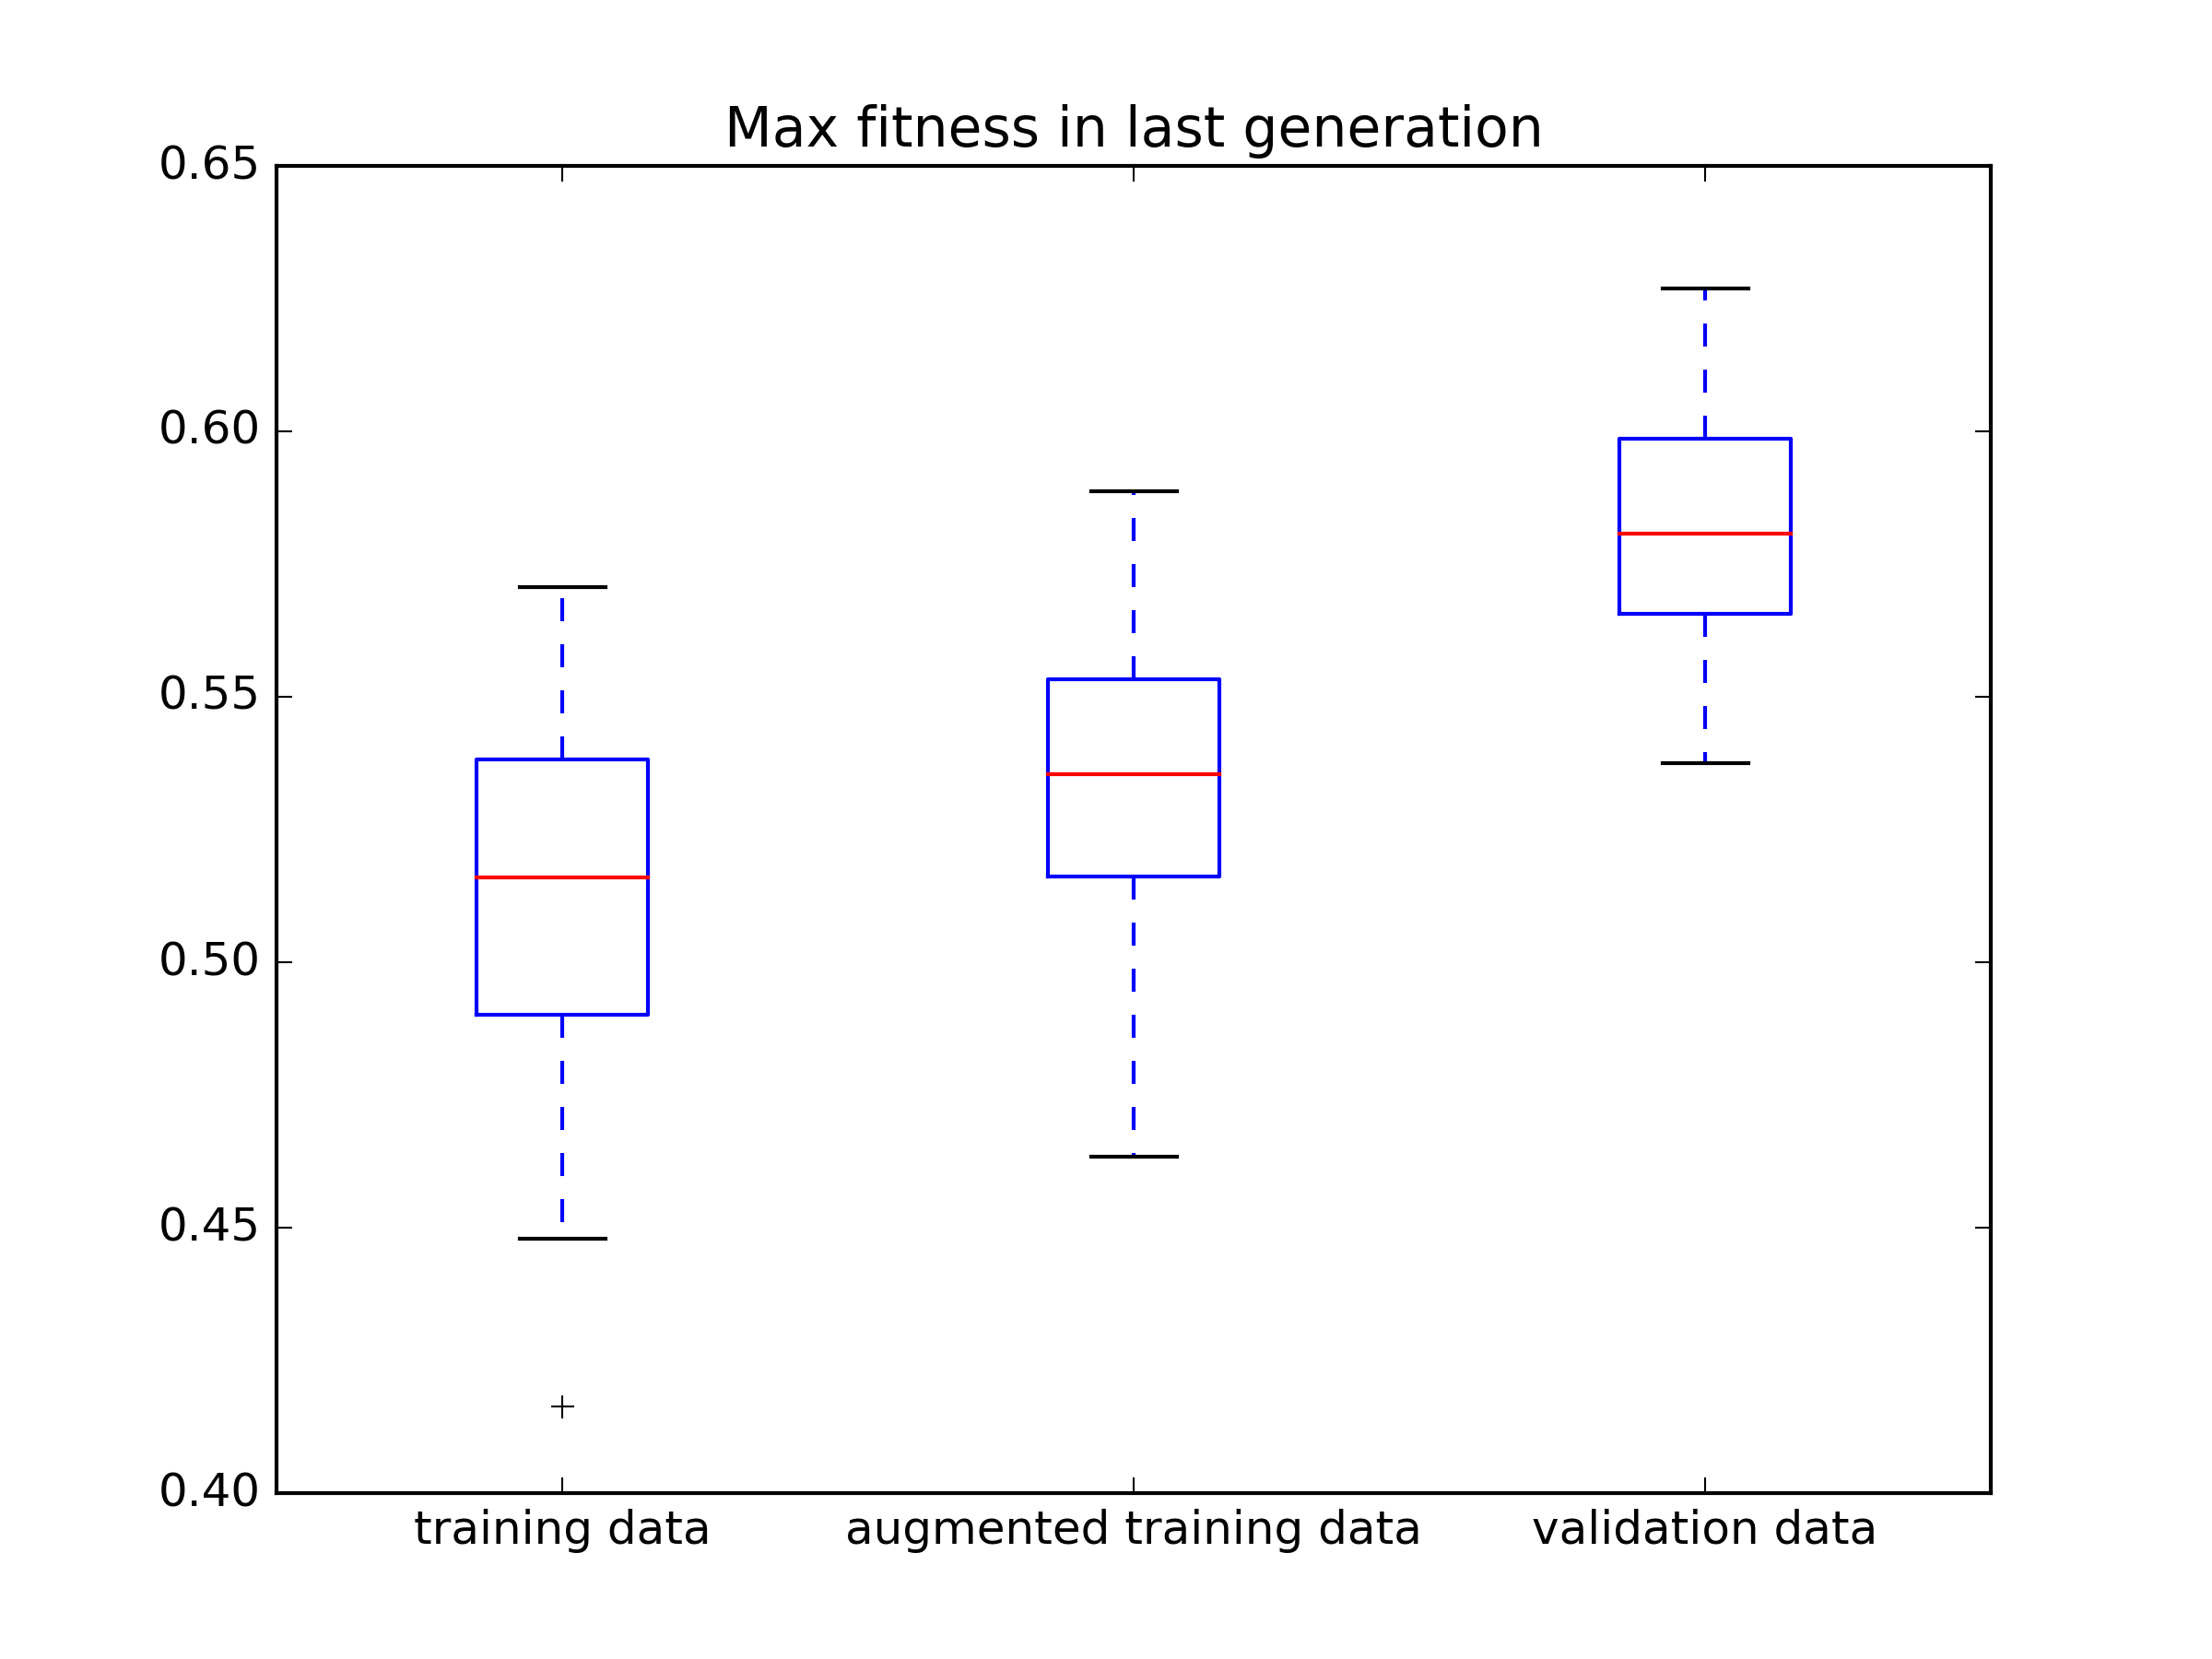
\includegraphics[width=1.0\textwidth]{exp3_fitness_box}
    \caption{Box plot of validation fitness values in final generation. The labels on the x-axis indicate which sound was used as target sound.}
    \label{fig:exp3_fitness_box}
\end{figure}
